\chapter{Graph}

\section{Fundamentals}

	\textbf{Curious Property of DFS:} 
	
	\begin{itemize}
	\item Given an undirected graph, assign each node to a set \textit{A}.
	\item Run a Depth-First-Search starting at any node.
	\item Whenever the DFS visits a new node N, remove N from \textit{A} and add it to the path set \textit{P}.
	\item Whenever the DFS backtracks from node N, remove N from the path and add it to set \textit{B}.
	\item Repeat until $|A| = |B|$. Which \textbf{will always occur}, because, in each operation, \textit{A} decreases by one and \textit{B} keeps it value. 
	Or, \textit{B} decreases by one and \textit{A} keeps it value.
	\item The DFS guarantees that \textit{A} and \textit{B} never have neighbouring nodes. 
	Because the set of nodes in Path \textit{P} separates them.
	\end{itemize}
	
	\kactlimport{dfs.cpp}

	\kactlimport{bfs.cpp}

\section{Network flow}

	In optimization theory, maximum flow problems involve finding a 
	feasible flow through a flow network that obtains the maximum possible flow rate. 

	\kactlimport{dinic.cpp}
	
	\kactlimport{dinitz.cpp}

	% for notebook generation
    \vspace{6pts}

	\subsection{Matching with Flow}

		By modeling a bipartite graph, with some Vertices (that will choose a match) to be on the L graph and some Vertices (that will be chosen) on the R.
		Set the correct capacities for these edges and also for the edges that connects the sink and source. After this modeling
		and running the dinic max flow algorithm, one will generate a possible matching (if it is possible).

		A special case of matching is the perfect matching, which includes all vertices from the bipartite graph L and R.

		A maximum matching has the maximum cadinality. A perfect matching is a maximum matching. 
		But the opposite is not necessarity true.

		It's possible to access dinic.edges, which is a vector that contains all edges and also its respective attributes, 
		like the \textit{flow} passing through each edge. Remember to consider that negative flow exist for reverse edges.

	\subsection{Minimum Cut}

		In computer science and optimization theory, the max-flow min-cut theorem states that, in a flow network, 
		the maximum amount of flow passing from the source to the sink is equal to the total weight of the edges 
		in a minimum cut, i.e., the smallest total weight of the edges which if removed would disconnect the source from the sink. 

		Let's define an s-t cut C = (S-component, T-component) as a partition of V $\in$ G such that 
		source s $\in$ S-component and sink t $\in$ T-component. Let's also define a cut-set of C to be the set 
		(u, v) $\in$ E | u $\in$ S-component, v $\in$ T-component such that if all edges in the cut-set of C are removed,
		the Max Flow from s to t is 0 (i.e., s and t are disconnected). The cost of an s-t cut C is defined by the sum
		of the capacities of the edges in the cut-set of C.

		The by-product of computing Max Flow is Min Cut! After Max Flow algorithm stops, we run graph traversal (DFS/BFS)
		from source s again. All reachable vertices from source s using positive weighted edges in the residual graph belong
		to the S-component. All other unreachable vertices belong to the T-component. All edges connecting the S-component to
		the T-component belong to the cut-set of C. The Min Cut value is equal to the Max Flow value.
		This is the minimum over all possible s-t cuts values.

	\subsection{Minimum Vertex Cover}

		The \textbf{Konig's Theorem} describes an equivalence between the maximum matching
		problem and the minimum vertex cover problem in bipartite graphs.

		Therefore, the value for the maximum flow in a bipartite graph is the same value as the number of nodes in a minimum vertex cover.

		To retrieve the set of vertices of the minimum vertex cover:
		\begin{itemize}
			\item Give orientation to the edges, matched edges start from the right side of the graph to the left side, and free edges start from the left side of the graph to the right side.
			\item Run DFS from unmatched nodes of the left side, in this traversal some nodes will become visited, others will stay unvisited.
			\item The MVC nodes are the visited nodes from the right side, and unvisited nodes from the left side.
		\end{itemize}

		$$ MVC = Visited_{Right} \cup Unvisited_{Left} $$

		\kactlimport{min-vertex-cover.cpp}
	
	% for notebook generation
	\vspace{5pts}

	\subsection{Maximum Independent Set}

		A \textbf{Independent Set} is a subset of nodes, in which all pairs {$u$, $v$} in the subset are not adjacent (There is no direct edge between nodes $u$ and $v$).
		
		A \textbf{Maximum Independent Set} is a \textit{Independent Set} with maximum cardinality;

		The \textbf{Maximum Independent Set} is complementar to the \textbf{Minimum Vertex Cover}.

		$$ MaxIS = all_{Vertices} \setminus MVC $$

		Therefore, to acquire the \textbf{Maximum Independent Set}, run the MVC algorithm and subtract them from the set of vertices and it will end up with the maxIS.

\section{Minimum Cost Matching}
	
	\subsection{Minimum Cost with Dinitz}

		\kactlimport{min-cost-dinitz.cpp}

	\subsection{Hungarian}

		Solves the \textbf{Assignment Problem:}

		There are several standard formulations of the assignment problem (all of which are essentially equivalent). Here are some of them:

		There are $n$ jobs and $n$ workers. Each worker specifies the amount of money they expect for a particular job.
		Each worker can be assigned to only one job. The objective is to assign jobs to workers in a way that minimizes the total cost.

		Given an $n \times n$ matrix $A$, the task is to select one number from each row such that exactly 
		one number is chosen from each column, and the sum of the selected numbers is minimized.

		Given an $n \times n$ matrix $A$, the task is to find a permutation $p$ of length $n$ such that the value
		$\sum A[i]\left[p[i]\right]$ is minimized.

		Consider a complete bipartite graph with $n$ vertices per part, where each edge is assigned a weight.
		The objective is to find a perfect matching with the minimum total weight.

		It is important to note that all the above scenarios are "square" problems, meaning both dimensions are always equal to
		$n$. In practice, similar "rectangular" formulations are often encountered, where $n$ is not equal to 
		$m$, and the task is to select $\min(n,m)$ elements. However, it can be observed that a "rectangular" 
		problem can always be transformed into a "square" problem by adding rows or columns with zero or infinite values, respectively.

		We also note that by analogy with the search for a minimum solution, one can also pose the problem of finding a maximum solution. 
		However, these two problems are equivalent to each other: it is enough to multiply all the weights by $-1$.

		\kactlimport{hungarian.cpp}
	
\section{Coloring}

	\textbf{Chromatic Number} is the \textit{minimum} number of colors to color all the vertices, so that no two adjacent vertices have the same color.

	\textbf{Chromatic Polynomial} $P(K)$ is the number of ways to color a graph with $K$ colors. 

	A \textbf{k-coloring} is the same as a partition of the vertex set into $k$ independent sets, and the terms \textit{k-partite} and \textit{k-colorable} have the same meaning.
	
	A \textit{clique} of size $N$ will force the Chromatic Number to be at least $N$. It is a \textit{lower bound}.

	The \textbf{maximum vertex degree $(+1)$} in an undirected graph will be the \textit{upper bound} on the Chromatic Number.

	\textbf{2-colorable graphs} are exactly the bipartite graphs.

	\textbf{Four color theorem} states that every planar graph can be 4-colored. 
	A planar graph is a graph that can be drawn in a 2D plane without edges intersecting.

	\subsection{Compute the Chromatic Number}
	
		\kactlimport{chromatic-number.cpp}

\section{Shortest Paths}

	For weighted directed graphs

	\subsection{Dijkstra}

		Single Source and there \textbf{cannot} be any negative weighted edges. 

		\kactlimport{dijkstra.cpp}

		By inverting the sorting order, Dijkstra can be modified for the opposite operation: \textit{longest paths}.

		Furthermore, Dijkstra be extended to keep track of more information, such as:

		\begin{itemize}
			\item how many minimum-price routes are there? (modulo $10^9+7$)
			\item what is the minimum number of flights in a minimum-price route?
			\item what is the maximum number of flights in a minimum-price route?
		\end{itemize}

		\kactlimport{extendedDijkstra.cpp}

	\subsection{Bellman-Ford}

		Single Source and it \textbf{supports} negative edges

		\textbf{Conjecture:} After at most n-1 (Vertices-1) iterations, all shortest paths will be found.
		
		\kactlimport{bellman-ford.cpp}

		By iterating once more, one can check if the last iteration reduced once again any distance. If so, it means that
		there must be a negative cycle, because the shortest distance should have been found before elseway.
		
		To retrieve the negative cycle itself, one can keep track of the last vertice that reaches a considered vertice

		\kactlimport{bellman-ford-cycle.cpp}
	
	% for notebook generation
	\vspace{7pts}

	\subsection{Floyd Warshall}

	All-Pair Shortest Paths

	\kactlimport{floyd-warshall.cpp}

\section{Eulerian Path}

	An \textit{Eulerian trail (or Eulerian path)} is a trail in a finite graph that visits every edge exactly once 
	(allowing for revisiting vertices). Similarly, an \textit{Eulerian circuit or Eulerian cycle} is an Eulerian trail 
	that starts and ends on the same vertex. 

	\textbf{Euler's Theorem:} A connected graph has an Euler cycle if and only if every vertex has even degree.

	An \textbf{Eulerian Graph} is a graph with an eulerian circuit, which implies that it is connected and 
	also all vertices have even degree.

	\begin{center}
	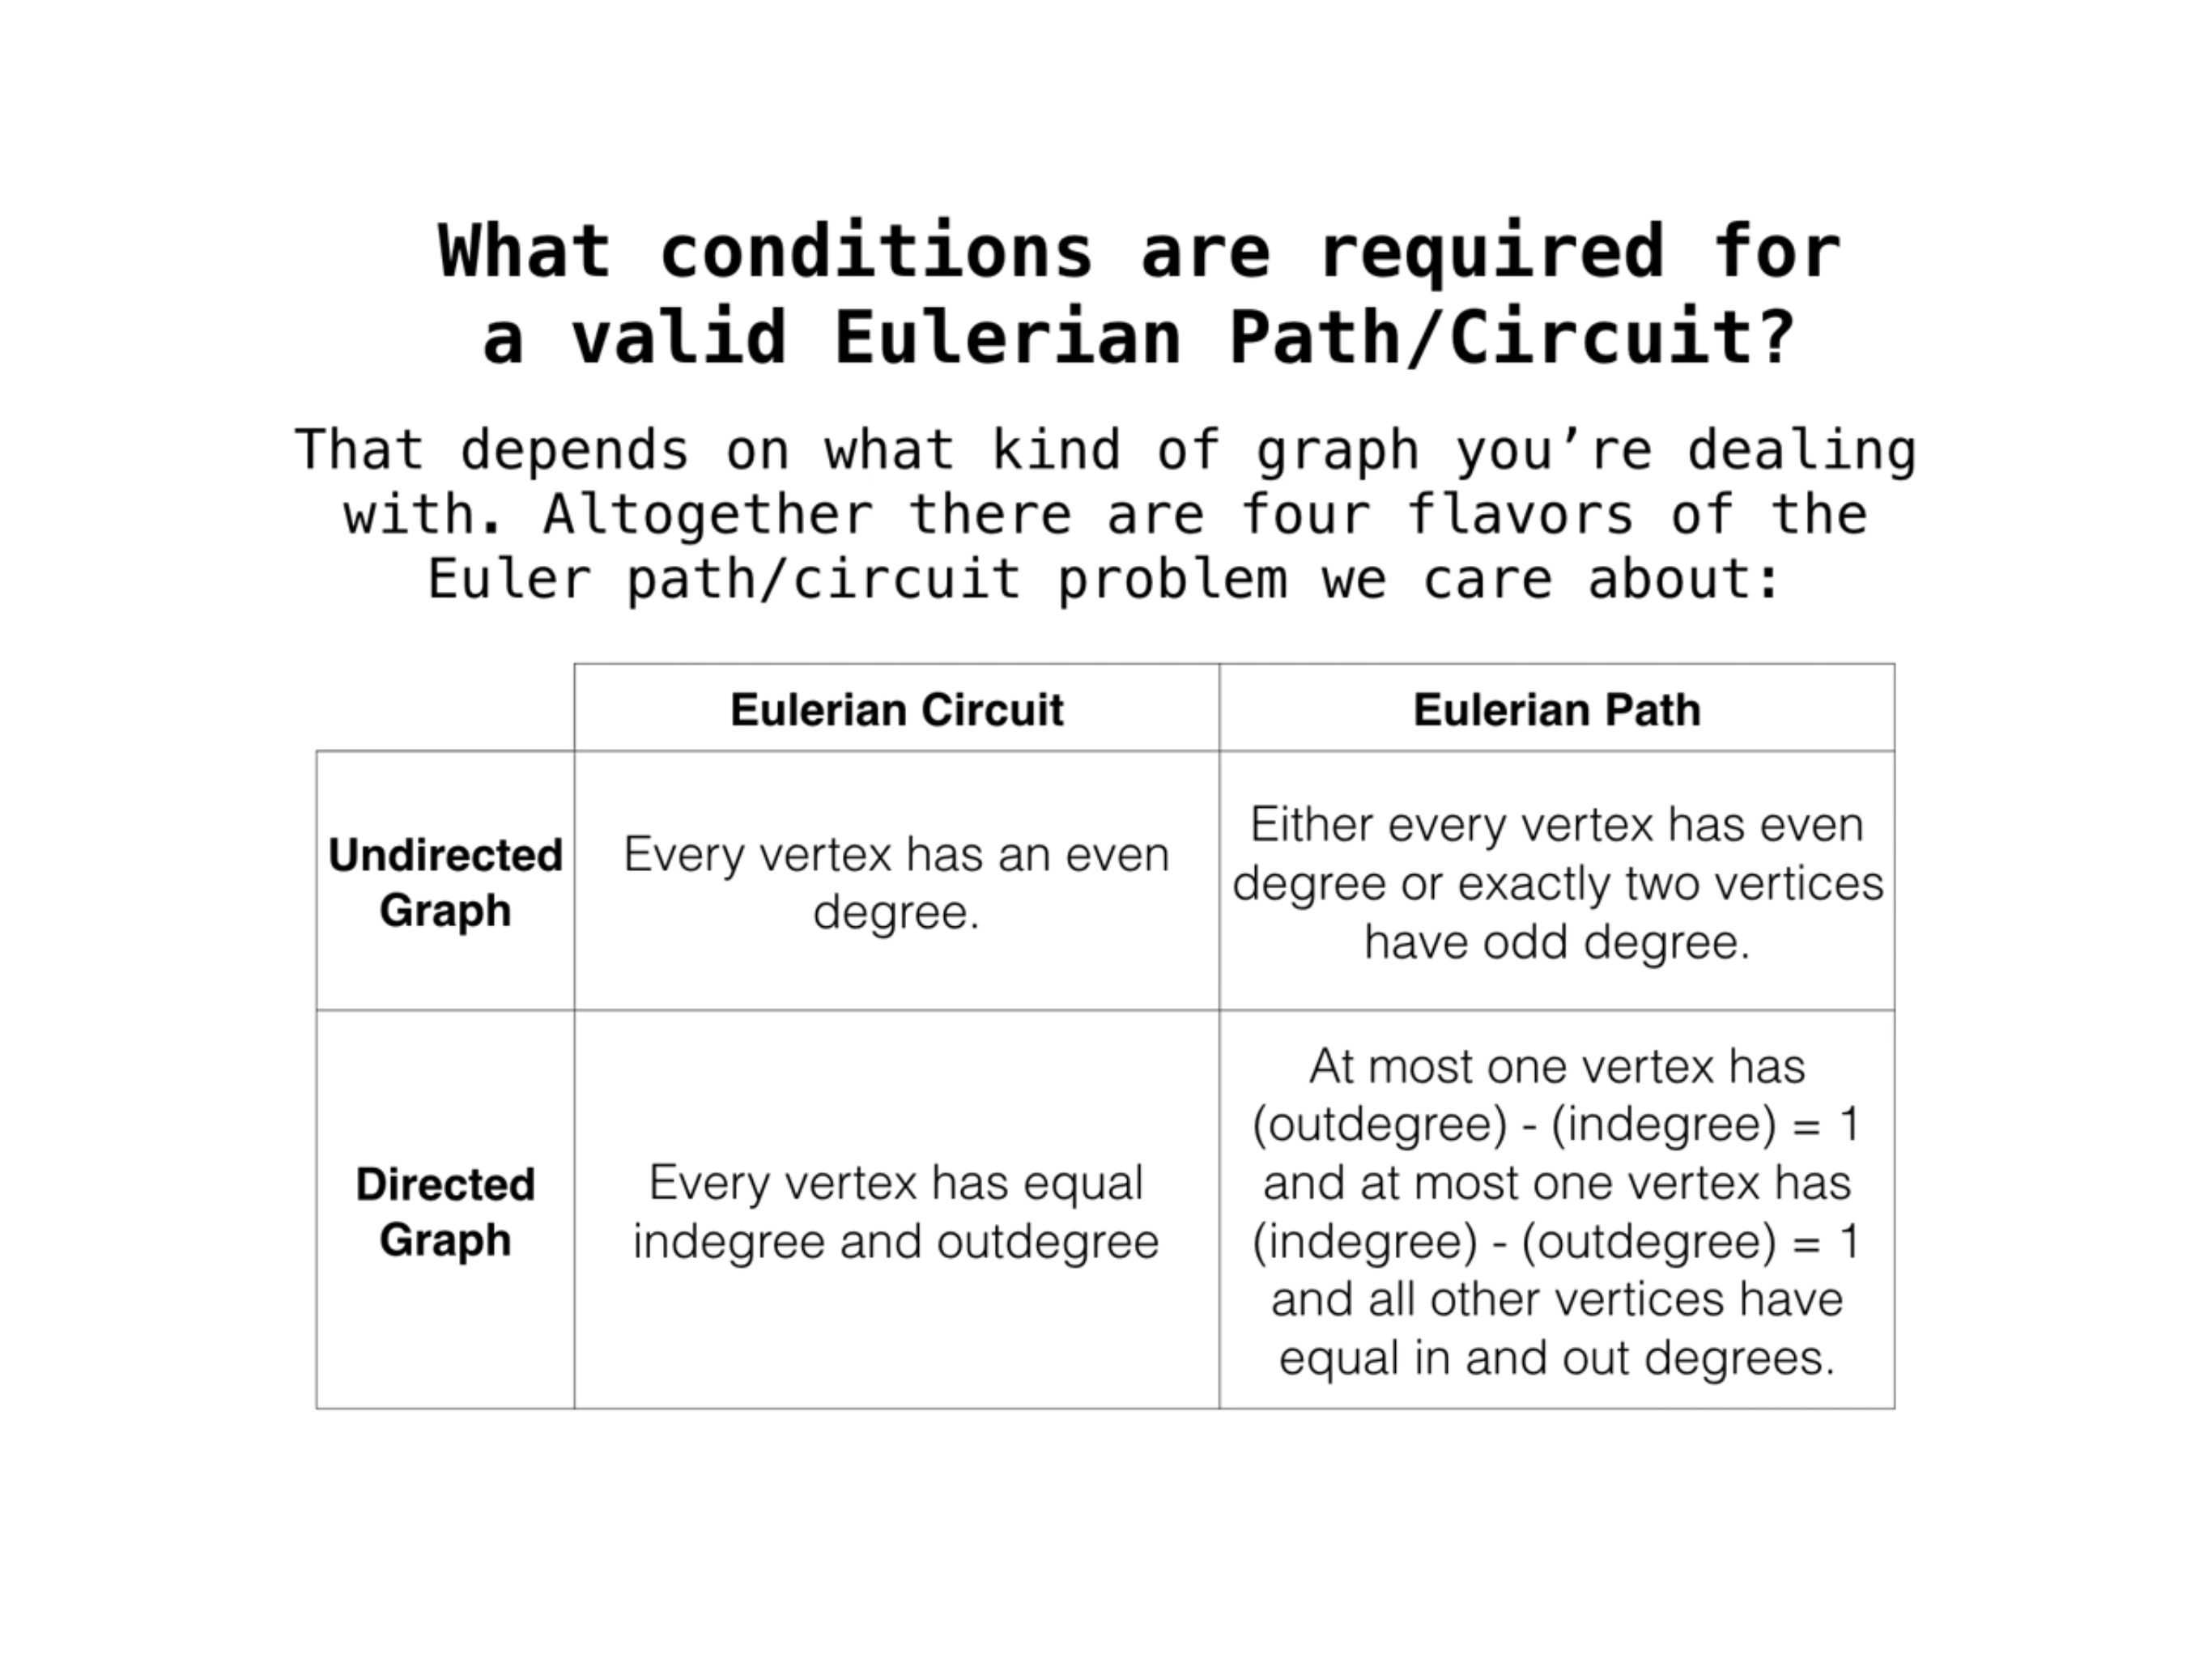
\includegraphics[scale=.1, keepaspectratio]{content/graph/Eulerian-Path-Existence.png}
	\end{center}

	If there are extra edges, which ones can be removed to generate a maximum size euler path?

	\textbf{Answer:} In an undirected graph, one can remove the ones connecting two \textit{odd} degree 
	nodes, turning then into \textit{even} ones. Do this until there are less or equal than 2 \textit{odd} degree nodes. 

	\kactlimport{hierholzer.cpp}

\section{Undirected Graph}

	Bridges and Articulation Points are concepts for undirected graphs!
	
	\subsection{Bridges (Cut Edges)}

		Also called \textbf{isthmus} or \textbf{cut arc}.
		
		A back-edge is never a bridge!
		
		A \textbf{lowlink} for a vertice $U$ is the closest vertice to the root reachable using only span edges and a \textit{single} back-edge, starting in the subtree of $U$.
		
		After constructing a DFS Tree, an edge (u, v) is a bridge $\iff$ there is no back-edge from $v$ (or a descendent of $v$) to $u$ (or an ancestor of $u$)
		
		To do this efficiently, it's used $tin[i]$ (entry time of node $i$) and $low[i]$ (minimum entry time considering all nodes that can be reached from node $i$).
		
		In another words, a edge (u, v) is a bridge $\iff$ the low[v] > tin[u].

		\kactlimport{bridges.cpp}

	\subsection{Bridge Tree}

	After merging \textit{vertices} of a \textbf{2-edge connected component} into single vertices, and leaving only bridges, one can generate a Bridge Tree.

	Every \textbf{2-edge connected component} has following properties:

    \begin{itemize}
		\item For each pair of vertices {A, B} inside the same component, there are at least 2 distinct paths from A to B (which may repeat vertices).
	\end{itemize}

	\kactlimport{bridgeTree.cpp}
	
	\subsection{Articulation Points} 

	One Vertice in a graph is considered a Articulation Points or Cut Vertice if its removal in the graph will generate more disconnected components

	\kactlimport{articulation.cpp}

	\subsection{Block Cut Tree}

	After merging \textit{edges} of a \textbf{2-vertex connected component} into single vertices, one can obtain a block cut tree.

	2-vertex connected components are also called as biconnected component
	
	Every bridge by itself is a biconnected component

	Each edge in the block-cut tree connects exactly an Articulation Point and a biconnected component (bipartite graph)

	Each biconnected component has the following properties:

	\begin{itemize}
		\item For each pair of edges, there is a cycle that contains both edges
		\item For each pair of vertices {A, B} inside the same connected component, there are at least 2 distinct paths from A to B (which do not repeat vertices).
	\end{itemize}

	\kactlimport{blockCutTree.cpp}
	
	% for notebook generation
	\newpage

	\subsection{Strong Orientation}

	A \textbf{strong orientation} of an undirected graph is an assignment of a direction to each edge that makes it a strongly connected graph.
	That is, after the orientation we should be able to visit any vertex from any vertex by following the directed edges.

	Of course, this cannot be done to every graph. Consider a \textbf{bridge} in a graph.
	We have to assign a direction to it and by doing so we make this bridge "crossable" in only one direction.
	That means we can't go from one of the bridge's ends to the other, so we can't make the graph strongly connected.

	Now consider a DFS through a bridgeless connected graph. Clearly, we will visit each vertex.
	And since there are no bridges, we can remove any DFS tree edge and still be able to go from below the edge to
	above the edge by using a path that contains at least one back edge. 
	From this follows that from any vertex we can go to the root of the DFS tree. 
	Also, from the root of the DFS tree we can visit any vertex we choose. We found a strong orientation!

	In other words, to strongly orient a bridgeless connected graph, 
	run a DFS on it and let the DFS tree edges point away from the DFS root and all other edges 
	from the descendant to the ancestor in the DFS tree.

	% https://cses.fi/problemset/result/8270539/

	The result that bridgeless connected graphs are exactly the graphs that have strong orientations is called \textbf{Robbins' theorem}.

		\subsubsection{Acyclic Graph Orientation}

			\textbf{Problem:} Given an undirected graph, your task is to choose a direction for each edge so that the resulting directed graph is acyclic.

			\textbf{Solution:} Do a dfs tree, every span-edge is oriented according to the dfs transversal,
			and every back-edge is oriented contrary to the dfs transversal

			% https://cses.fi/problemset/result/8476041/

\section{Directed Graph}

	\subsection{Topological Sort}

	Sort a directed graph with no cycles (DAG) in an order which each source of an edge is visited before the sink of this edge.

	Cannot have cycles, because it would create a contradition of which vertices whould come before.

	It can be done with a DFS, appending in the reverse order of transversal. Also a stack can be used to reverse order	

	\kactlimport{toposort.cpp}

	% for notebook generation
    \vspace{5pts}
	
	\subsection{Kosaraju}

	A Strongly Connected Component is a maximal subgraph in which every vertex is reachable
	from any vertex inside this same subgraph.

	A important \textit{property} is that the inverted graph or transposed graph has the same SCCs
	as the original graph.

	\kactlimport{kosaraju.cpp}

	\subsection{2-SAT}
	
		SAT (Boolean satisfiability problem) is NP-Complete.

		2-SAT is a restriction of the SAT problem, in 2-SAT every clause has exactly two variables:
		$ (X_1 \vee X_2) \wedge (X_2 \vee X_3) $

		Every restriction or implication are represented in the graph as directed edges.

		The algorithm uses kosaraju to check if any ($X$ and $\neg{X}$) are in the same Strongly Connected Component 
		(which implies that the problem is impossible). 

		If it doesn't, there is at least one solution, which can be generated using the topological sort of the same kosaraju 
		(opting for the variables that appers latter in the sorted order)

		\kactlimport{2sat.cpp}

\section{Minimum Spanning Tree}

\subsection{Undirected Minimum Spanning Tree}

	A \textbf{minimum spanning tree (MST)} or minimum weight spanning tree is a subset of the edges
	of a connected, edge-weighted undirected graph that connects all the vertices together,
	without any cycles and with the minimum possible total edge weight.
	That is, it is a spanning tree whose sum of edge weights is as small as possible.

	\kactlimport{kruskal.cpp}

\subsection{Directed Minimum Spanning Tree}

	A \textbf{spanning arborescence of minimum weight}, sometimes called an \textbf{optimum branching},
	is the directed analog of the \textit{minimum spanning tree problem}.

	\subsubsection{Edmonds' algorithm with Tarjan's optimization}

	\kactlimport{directed-mst.cpp}

\section{Trees}

	\kactlimport{lca.cpp}

	\kactlimport{binary-lifting.cpp}

\subsection{Small To Large}

	Count the number of occurences of each color in every subtree in $O(n log(n))$.

	\kactlimport{sack.cpp}
% \section{Math}
